\chapter{Search for invisibly decaying VBF produced Higgs bosons in Run 1 prompt data}
\label{chap:prompt}
%??Introduction to selection and challenges of jets+met, e.g. trigger, QCD
As described in \ChapterRef{chap:theory}, searches for invisible Higgs boson decays are well motivated by their sensitivity to new physics, such as \ac{DM}. Because the invisible branching of an \ac{SM} 125 GeV Higgs boson is very small, any observation made of invisible Higgs boson decays at the \LHC would be evidence for physics beyond the \ac{SM}. This chapter describes the search for invisible Higgs boson decays using data taken by CMS in 2012 with a promptly reconstructed trigger developed specifically for this analysis. The total integrated luminosity collected with this trigger that was certified for use in physics analyses was 19.5\invfb~.

This chapter will start by describing the trigger and event selection in detail, before explaining the techniques used for estimating the number of events passing the analysis selection from background processes. Systematic uncertainties will then be described, followed by the results of the analysis. This analysis was published in \ReferenceRef{Chatrchyan:2014tja}.

\section{Event selection}%??
\label{sec:promptsel}
%??describe backgrounds and motivate selection
In signal events it is expected that there will be two jets with a characteristic \ac{VBF} topology and a large amount of \MET. Several background processes, with significantly higher cross-sections than the signal process, can also produce events with these objects present. It is therefore necessary to design selection criteria to remove as many of these background events from the analysis as possible.

The most significant of these background processes is the production of a vector boson in association with jets. Leptonic decays of \PW bosons and \PZ boson decays to neutrinos both produce \MET and, due to the approximately 1000 times higher cross-section for vector boson production than Higgs boson production, there are many events where the associated jets have a \ac{VBF}-like topology. %??relative cross-section
A further background process that can produce significant numbers of \ac{VBF}-like jets due to its very large cross-section is QCD production of multiple jets (``QCD multijets''). Whilst these multijet events have very little \MET from real invisible particles, it is possible for significant ``fake'' \MET to be caused by mismeasurement of the jets. The production of two vector bosons or top quarks can also lead to two jets and real \MET, although they have much lower cross-sections than the other background processes and their contribution is not as significant.

%??trigger requirements and design
\subsection{Trigger}
The trigger requirements can be viewed as the first stage of the event selection. Their primary role is to reduce the rate of events that must be recorded by the detector whilst retaining as many signal events as possible. To pass the \ac{L1} trigger selection events are required to have \MET$>40$ \GeV. Events are then required to have \METnoMU$>65$ \GeV and that at least one pair of jets in the event is \ac{VBF}-like to pass the \ac{HLT} selection. The \ac{VBF}-like requirements on the jets consist of requiring their $\eta$ separation, $\Delta\eta_{jj}$, be greater than 3.5, that they are in opposite forward/backward halves of the detector and that they have high invariant mass, $M_{jj}>800 \GeV$. The use of \METnoMU at trigger level ensures that events which are needed for the control regions used in the background estimation techniques described in \SectionRef{sec:promptbkg} are not rejected. Not requiring that the \ac{VBF}-like pair of jets also be the two highest \pt jets reduces inefficiencies caused by different \pt orderings in jets reconstructed by the trigger and by the offline reconstruction. 

As described in \SectionRef{sec:triggers} the decision whether to keep an event must be made very rapidly, and as a result the object reconstruction algorithms used are less sophisticated, and the available detector resolution is worse, than those offline. The trigger criteria have therefore been chosen to be as loose as possible whilst maintaining the required rate reduction. The efficiency for events to pass the trigger as a function of their values of several offline variables is shown in \FigureRef{fig:prompttrigplots}.

\begin{figure}
  \subfloat[]{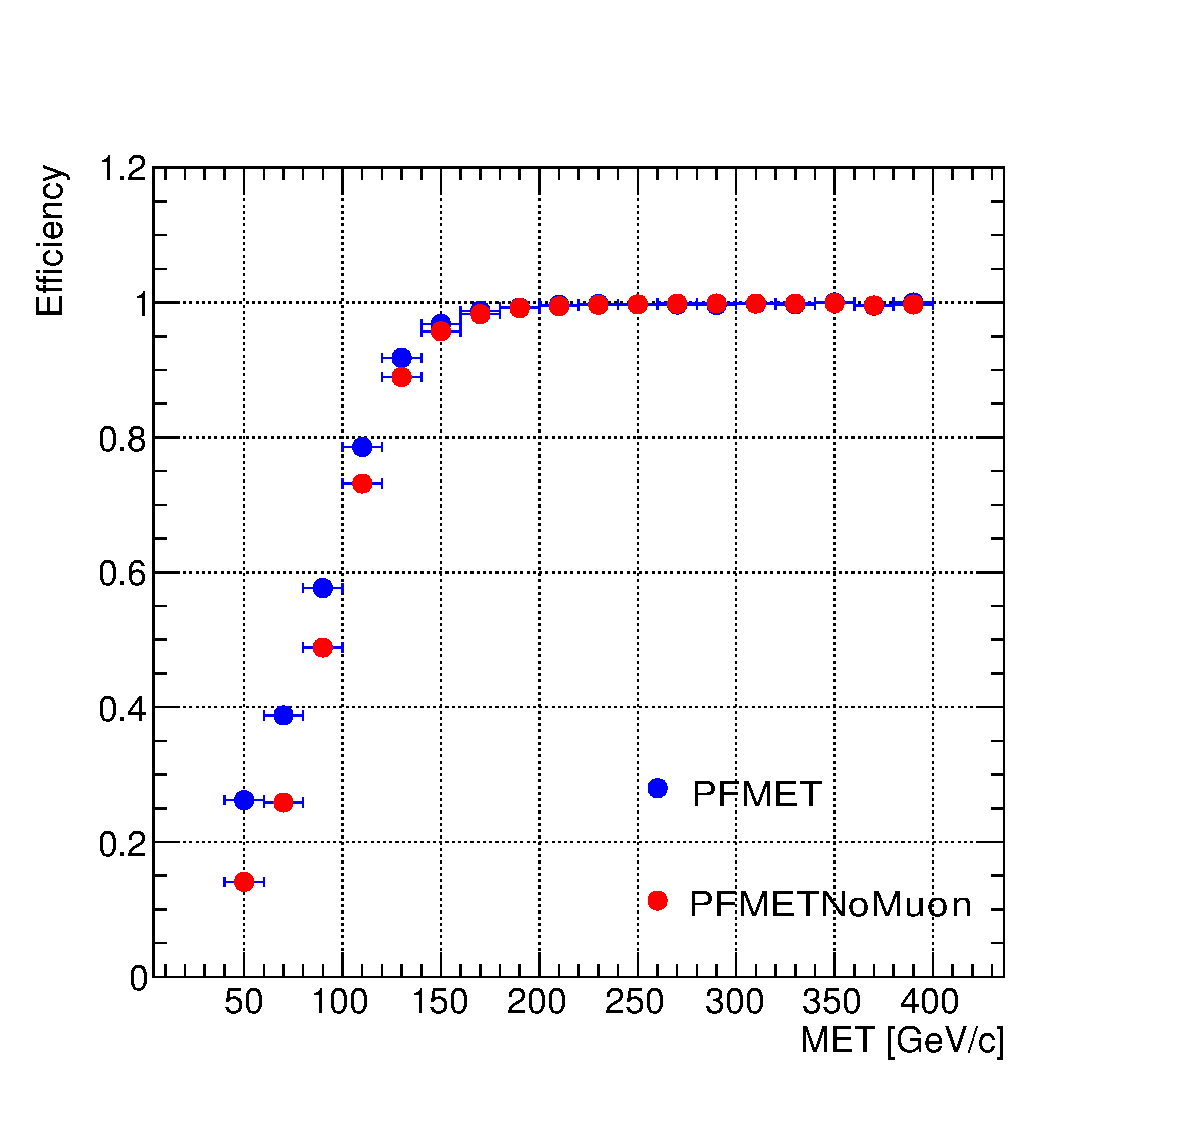
\includegraphics[width=.6\largefigwidth]{plots/prompt/TrigEff_SingleMu_L1ETM40.pdf}}
  \subfloat[]{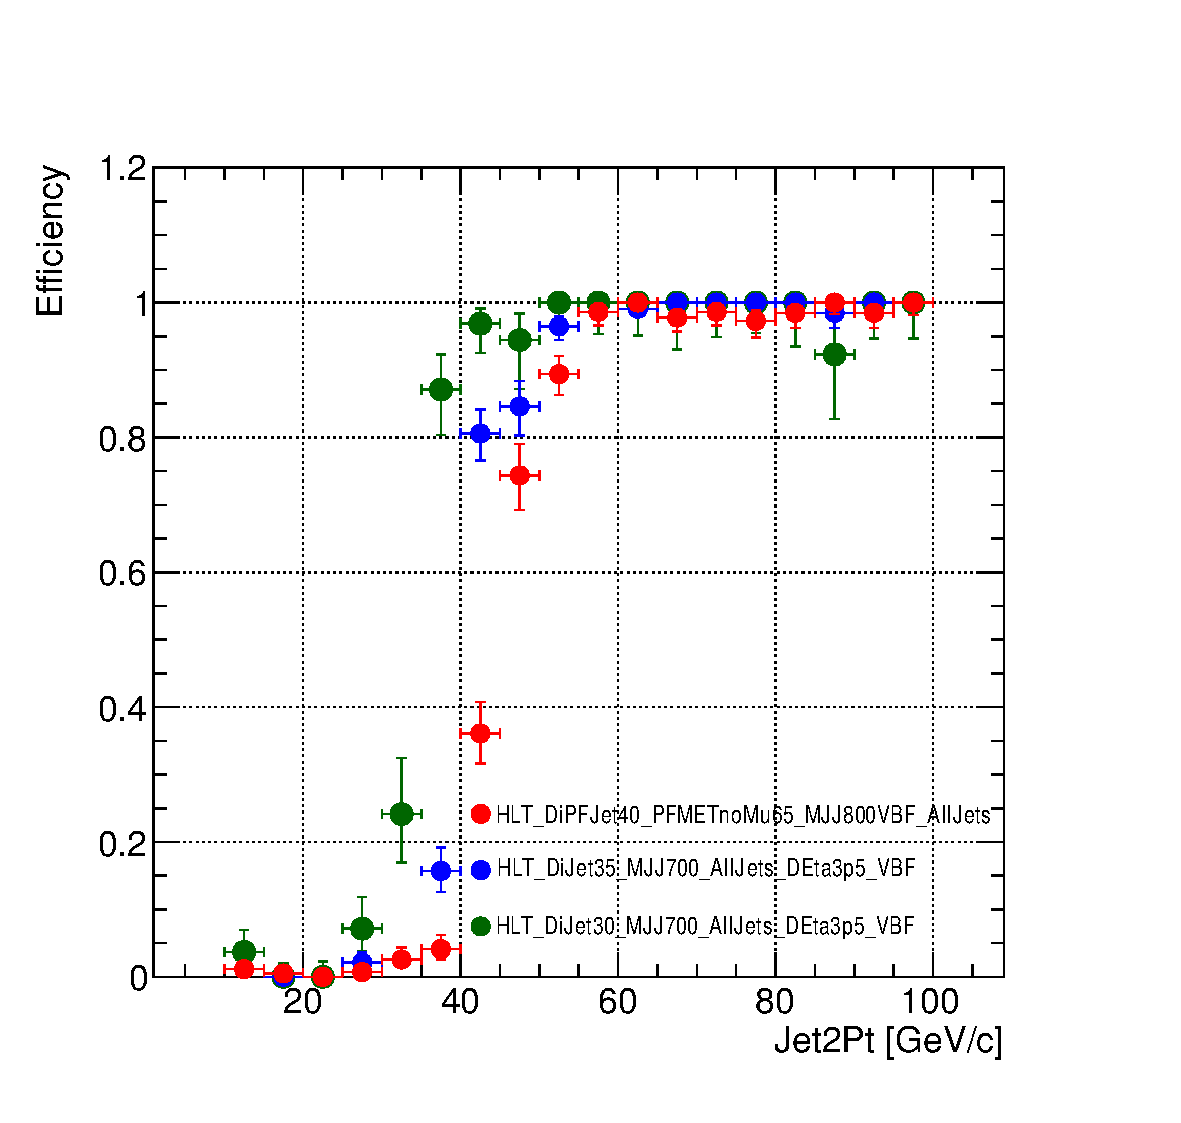
\includegraphics[width=.6\largefigwidth]{plots/prompt/TrigEff_SingleMu_Jet2Pt.pdf}}

  \subfloat[]{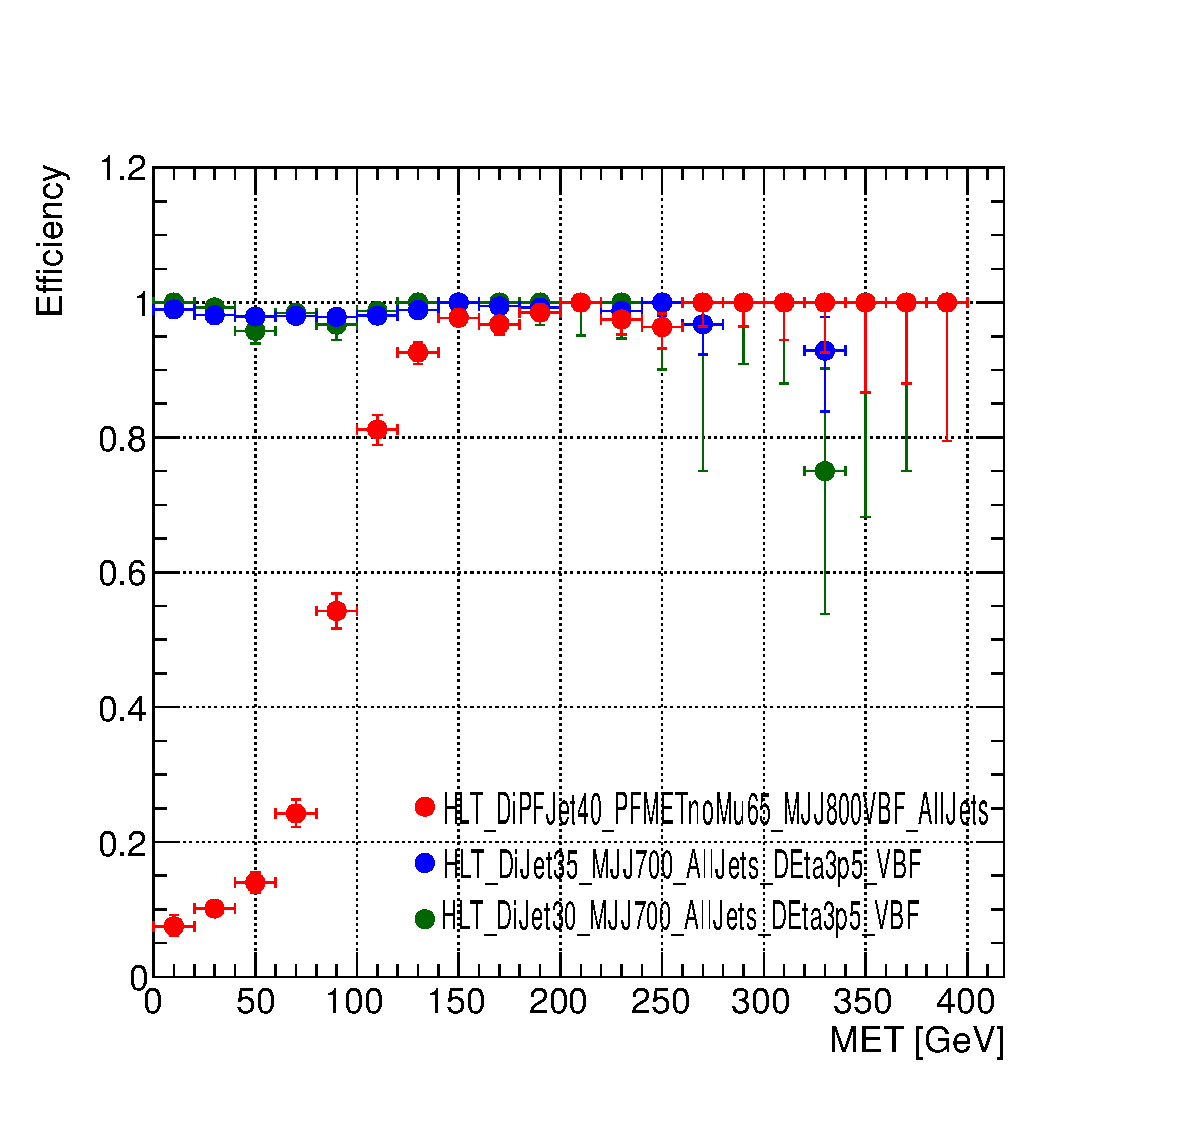
\includegraphics[width=.6\largefigwidth]{plots/prompt/TrigEff_SingleMu_MET.pdf}}
  \subfloat[]{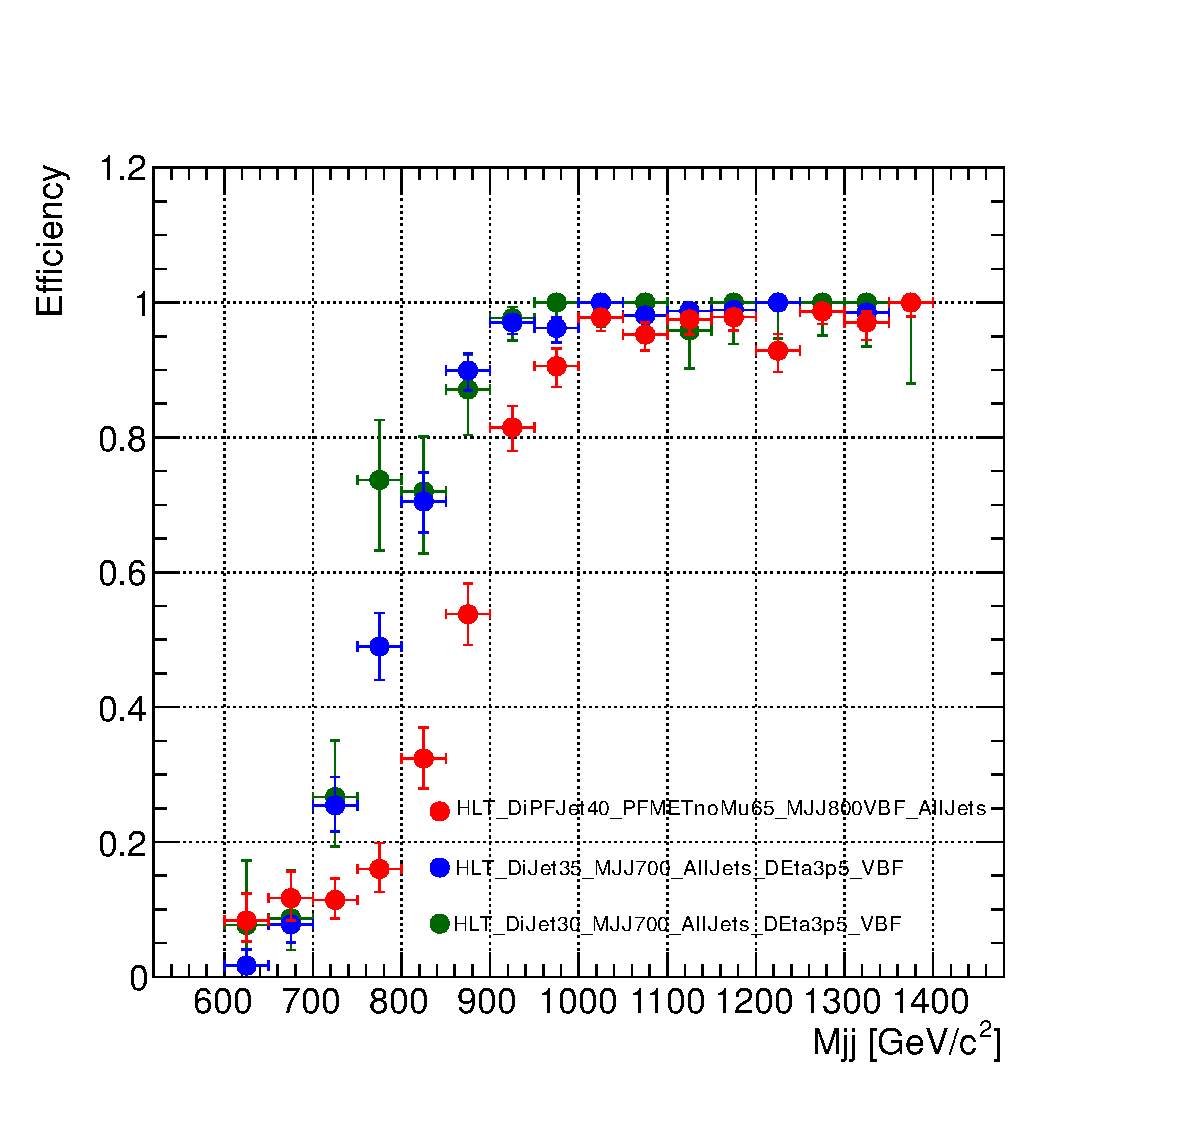
\includegraphics[width=.6\largefigwidth]{plots/prompt/TrigEff_SingleMu_Mjj.pdf}}
  \caption{The efficiency for events to pass the stages of the trigger criteria as a function of their values of several offline variables. (a) \ac{L1} trigger efficiency as a function of offline \MET and \METnoMU, (b) \ac{HLT} efficiency as a function of second highest offline jet \pt, (c) \ac{HLT} efficiency as a function of offline \MET, (d) \ac{HLT} efficiency as a function of $M_{jj}$.}
  \label{fig:prompttrigplots}
\end{figure}
%??trigger efficiency plots

%??selection and motivation
%??lepton and jet pt requirements

\section{Background estimation}%??
\label{sec:promptbkg}

\subsection{W$\rightarrow e\nu$+jets}%??
\label{sec:promptwenu}

\subsection{W$\rightarrow \mu\nu$+jets}%??
\label{sec:promptwmunu}

\subsection{W$\rightarrow \tau\nu$+jets}%??
\label{sec:promptwtaunu}

\subsection{Z$\rightarrow \nu\nu$+jets}%??
\label{sec:promptznunu}

\subsection{QCD}%??
\label{sec:promptQCD}

\subsection{Minor backgrounds}%??
\label{sec:promptminor}

\section{Systematic uncertainties}%??
\label{sec:promptsyst}
%??Systematics

\section{Results}%??
\label{sec:promptresults}
